En flip-flop kan lagre én bit, det er ikke særlig nyttig.
La oss sette sammen flere av dem så vi for et n-bit register.
\\\\
Ved å bruke D-latches hvor D inngangene er koblet til et binært input og
klokkeinngangen er delt, kan vi lage et register som kan lagres med
et klokkesignal.
\begin{figure}[H]
  \caption{4bit register laget av D-Latches.}
  \centering
  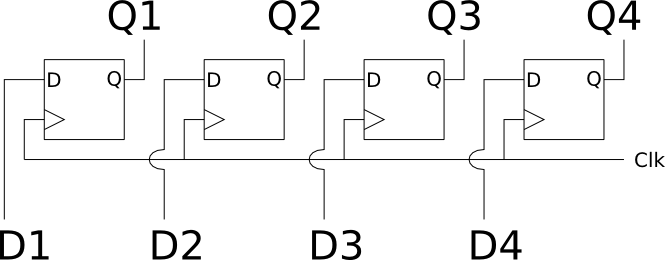
\includegraphics[width=\textwidth]{./img/register}
\end{figure}
Klokken er ikke nødvendigvis en puls.
Tenk på det som en 'lagre knapp' som lagrer dataen.
